\openingarticle
\def\ppages{\pagerange{Takkou:firstpage}{Takkou:lastpage}}
\def\shorttitle{Archaeological History of Zakynthos}
\def\maintitle{A Discourse on the Archaeological History of Zakynthos: Alternative Approaches}
\def\shortauthor{Richard Takkou, Sonja Dobroski }
%--------------------------------------------------------------
\mychapter{\maintitle}
\begin{center}
	{\Large\scshape
	Richard Takkou\footnote{\href{https://oxford.academia.edu/RichardTakkou}{Richard Takkou} started his archaeological career as a keen volunteer at the age of 25. His first career involved working in multiple roles in the international development (ID) sector. In his last ID role, he worked for the United Nations Developing Program (UNDP) in their office in Athens, Greece, before deciding to turn towards his beloved discipline -- Archaeology. He completed his undergraduate studies at UCL in 2013, specialising in Mesoamerican archaeology, and gained an MSt at the University of Oxford (2015), specialising in Maritime Archaeology. He has been published in the archaeological journal \textit{PIA} (Papers of the Institute of Archaeology) in 2014 and is currently working towards an archaeological PhD at the University of Nottingham. In addition, he co-owns Omni-Tech Archaeology, an anthropological and archaeological services company providing research, field schools and workshops.} \\
	{\normalfont\normalsize \href{mailto:takkou@hotmail.com}{takkou@hotmail.com}}\\[1em]	 
	{\normalfont\normalsize School of Archaeology, University of Oxford\\[1em]}
	Sonja Dobroski\footnote{\href{https://oxford.academia.edu/SonjaDobroski}{Sonja Dobroski} is new to the field, having recently completed her Master of Studies in Archaeology at the University of Oxford in 2015.  Sonja is a socio-cultural anthropologist, completing her B.A. in Anthropology and Native American Studies in 2009 at the University of Montana and her M.A. in American Indian Studies in 2012 at the University of California-Los Angeles. 
	Her venture into archaeology was inspired by a desire to take a material based approach to anthropological inquiry, specifically, studying hegemony as reflected in materials from the \nth{20} and \nth{21} centuries. She will begin her Doctorate in Socio-Cultural Anthropology at the University of St. Andrew's in September of 2016, focusing on the specific material outcomes of settler colonization. Her broad research interests include: Contemporary American Indian material culture, materiality, critical and settler colonial theory, identity politics, collective memory, oral history, and the digital humanities.  In addition, she co-owns Omni-Tech Archaeology, an anthropological and archaeological services company providing research, field schools and workshops.}\\ {\normalfont\normalsize\href{mailto:sldobroski@gmail.com}{sldobroski@gmail.com}
	}}\\[1em]
\end{center}
\vspace{3em}
\midarticle
%--------------------------------------------------------------	
\label{Takkou:firstpage}
\begin{myabstract}
The\marginnote{Abstract\\(in Greek see below)} archaeology on Zakynthos is sparse compared to that of the other Ionian Islands. This is due to a variety of circumstances - a lack of regional archaeological research and the archaeological record on the island showing a high degree of fragmentation and destruction due to a combination of war, seismic activity, and intensive land use or development, which has resulted in the loss of an unknown number of sites and/or artifacts. As a result of this loss, archaeological projects on the island of Zakynthos have produced an array of predominantly survey-based inquiries, which have been insufficient in ascertaining a comprehensive prehistoric interpretation of the Island. This paper explores the archaeological history of the island and presents preliminary fieldwork; completed in support of DPhil research scheduled for 2016, and conducted by the authors in August of 2015, on the coastal region of Katastari, Zakynthos (Greece). In addition, this paper responds to the difficult archaeological terrain on the island by exploring the potentials of a new community inclusive methodology for the region. 
	
\keywords[Keywords]{Zakynthos; Katastari; Survey; Oral History; Prehistory; Landscape archaeology.}
\end{myabstract}
	
%---------------------------------------------------------------------------------
	
	
%\section{Introduction}
\lettrine[nindent=0em,lines=3]{Z}{akynthos}, a small island in Greece, has received a great deal less archeological consideration historically than the other Ionian islands Ithaki and Kephallonia, and the adjacent western Peloponnese. To some degree, this may be the consequence of the way that Zakynthos is identifiably specified by Homer in the Iliad and the Odyssey as a major aspect of Odysseus' domain \parencite{VanWijngaarden_2013}. A great deal of the archeological examination on the Ionian islands has been impelled on by the quest for Homeric Ithaca \parencite[9]{Souyoudzouglou-Haywood_1999}. During the \nth{18}, \nth{19} and early \nth{20} centuries, interest in Homeric Greece manifested itself into archaeological projects aiming to find Homeric points of interest. For example, Schliemann, the finder of Troy, first attempted to locate Odysseus’ palace before setting out to find Troy. He and many others excavated ‘Homeric’ regions of Ithaki and Kephallonia (the two closest islands to Zakynthos) searching for the famed palace. Since Zakynthos had already been distinguished in ancient literature, it could not be Odysseus’ Ithaca and has, thusly, received less archeological consideration. Additionally, not very many visible archeological remains are obvious on the island. War and the combined influence of tectonics and eustasy contributed to forming the contemporary landscape. This paper presents an alternative, community-inclusive methodology, inspired by post-colonial critiques, to aid in the navigation and interpretation of this difficult archaeological history and terrain. The article focuses the application of this methodology through a discussion of the authors’ preliminary fieldwork conducted in August of 2015, where two potential archaeological sites were discovered in the coastal region of Katastari.
	
%	\section{Archaeological History}
	
Archaeological\marginnote{Archaeological History} research on the island has produced an array of predominantly survey-based inquiries. From these previous works, evidence suggests a significant Prehistoric presence on the island. The findings of \textcite{Riemann_1879}, \textcite{Benton_1933}, \textcite{Zapfe_1937}, \textcite{Sordinas_1970}, \textcite{Agallopoulou_1973}, and most recently the Zakynthos Archaeology Project (2006--2013) directed by Sotiriou and Van Wijngaarden, have shaped our current understanding of the prehistoric occupation on the island.  Other archaeologists have established the existence of a significant Hellenistic-Roman occupation \parencites{Daux_1958}{Mylonas_1991}{Kalligas_1993}{Arapoyianni_1991}{Arapoyianni_1992}.  The focus of this paper is on the prehistoric archaeological finds. 
	
Sylvia Benton’s fieldwork, conducted in 1931--1932, expanded upon the work of \textcite{Riemann_1879} and \textcite{Schmidt_1899}. She identified three Bronze Age sites on the island through the discovery of several surficial artifacts during her survey: an obsidian blade found on Cape Gerakini, Mycenaean style terracotta disks, and several Mycenaean pottery sherds and human skeletal remains found around a Tholos tomb near Akrotiri. Benton returned to the Alikanas-Akrotiri area the following year (1933--1934) with archaeologist, Hilda Lorimer where they found remnants of a Mycenaean house \parencite{Benton_1933}. These finds were never fully published and the artifacts taken were destroyed in an earthquake. \textcite{Sordinas_1970} surveyed the island between 1965 and 1966 and discovered several Paleolithic sites indicated by scattered lithics and pottery. Interestingly the only full-scale excavation of a pre-historic site was conducted by \textcite{Agallopoulou_1973}, who excavated 14 Mycenaean tombs in an ancient cemetery in the village of Kambi located \SI{30}{\kilo\metre} north of the town of Zakynthos. To date, the cemetery at Kambi remains the only archaeological site on Zakynthos that has been systematically excavated and fully published.
	
Currently, the work of the Zakynthos Archaeology Project, spearheaded by Van Wijngaarden, has synthesized this previous research and identified three larger research areas in which intensive survey and small-scale test excavations have been conducted. This has resulted in the discovery of thousands of prehistoric lithics and pottery sherds. A complete report of these finds has yet to be published as of the date of this publication. However, preliminary reports have been made available and have proved to begin to fill the archaeological gap in the known data record.
	
%\section{Fragmentation of the Archaeological Record Explained}
	
The\marginnote{Fragmentation of the Archaeological Record Explained} island has been colonised a myriad times since c.1500\BC, including by the Peloponnesians in 431\BC, Phillip II of Macedon in 217\BC and the Romans a few years later in 214\BC. After the Romans, came the Byzantines, who defended the island against the Visigoths and the Huns in 395\AD. Years later and after much plundering and looting, Zakynthos was the victim of barbarian attack yet again -- in 549\AD when the Visigoths, under Totilas, overran the island. The island suffered further attacks almost every year, mainly tormented by the Saracen pirates of Crete. By the time of the second crusade, in 1147\AD, Zakynthos was captured by the Venetian fleet of Domenico Michelo. The next 300 years consisted of ownership changes analogous to a game of musical chairs with the seat of power being transferred from the Venetians to the Neapolitans and then to the Florentines. This cycle of ownership continued until the Ottoman Turks decimated the island in 1480\AD. Two occurrences of Veneto-Turkish wars, three outbreaks of the black plague and unabated pirating of Zakynthian shores had left the islands rich archaeological heritage in a dire state by the time the British arrived in 1814\AD -- either by the dismantling of ancient structures in order to reuse material for newer structures or fortification of older structures, or by pure destruction by invading armies and pirates, usually manifested by fire.
	
The seismic activity and eustasy suffered by Zakynthos has been constant and consistent since the Middle Pleistocene \parencite[400]{Zelilidis_1998}. In the period from 25,000 to 4,000\BC the sea level has fluctuated between \SIrange[range-phrase=--]{120}{20}{\metre} below present level and, consequently, the landmass of Zakynthos was greater than it is today. Effectively, this means any early Mesolithic (8300--6000\BC) or Neolithic (6000--3200\BC) coastal settlements are now underwater \parencite[2172]{Ferentinos_2012}. Even though Zakynthos probably was attached to Kefalonia and Ithaki during parts of the Pleistocene, the group of islands remained insular and detached from the Greek mainland. Moreover, geological research indicates that the peninsula of Vasilikos was detached from the rest of Zakynthos and constituted a separate island until the end of the Bronze Age \parencite{Lambeck_2005}. The evidence of Paleolithic stone tools and Bronze Age pottery and lithics indicates that the island had a constant human presence from the Middle Paleolithic onwards \parencite[286]{Kourtessi-Philippakis_1999}. Nevertheless, the lack of stratigraphic deposits on the island make it difficult to assess these finds in a secure chronological framework. In all cases, the lithics and pottery have been found at open-air (surficial) sites or in off-site (back dirt) material. Further, in the region of Katastari, where there are some deposits of earth that are deep enough to be quantified in stratigraphic layers, farmers have worked this land for hundreds of years cultivating olives (\textit{Olea europaea}) and grapes (\textit{Vitis vinifer}) – the island’s largest exports. This has created a percolation of unearthed artifacts that have lost their stratigraphic context in the archaeological record and can only be dated via morphological similarities in regional pottery design (seriation). Certainly, the archaeological terrain of Zakynthos is complicated and fragmented, which calls archaeologists to continue to push methodological boundaries to meet these needs.
	
		%% this is figure 1
		\begin{figure}[!bt]
			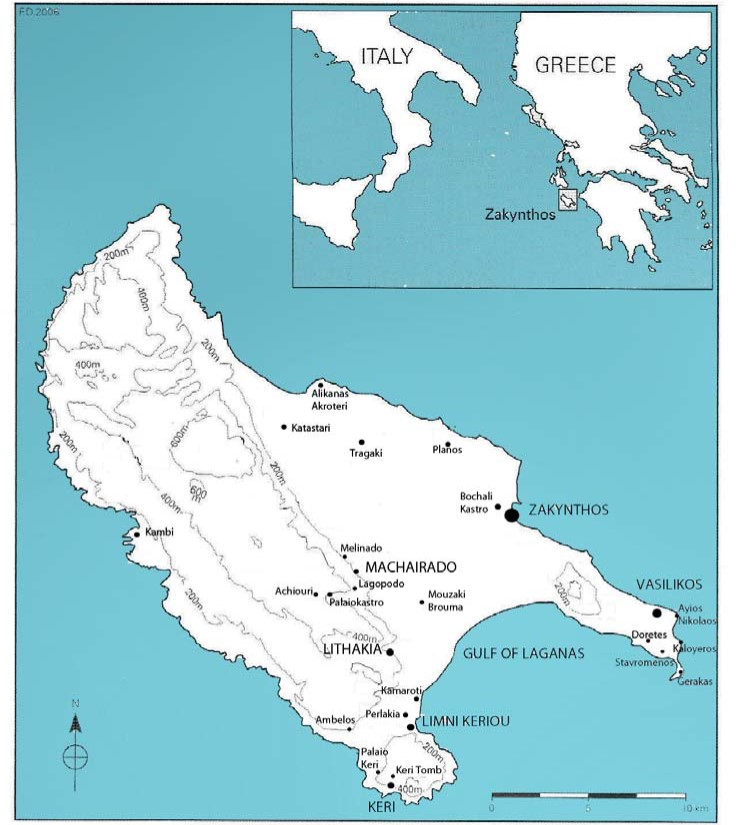
\includegraphics[width=\linewidth]{figures/takkou_dobroski_Fig1.jpg}
			\caption{Map of Zakynthos \parencite[128]{VanWijngaarden_2013}.}
			\label{fig:Takkou_Fig1}
		\end{figure}
		
%	\section{New Methodology}
	
Archaeological\marginnote{New Methodology} studies of ancient Greece seem an unlikely candidate for post-colonial critiques. Arguably, all archaeology in the \nth{21} century is of a post-colonial context and as such, to a certain extent, merits this lens. Previous approaches in the region often disenfranchised local communities from participating in the archaeological interpretation and heritage of the island by ignoring locally derived knowledge. Local communities have internalised a distinct historical understanding of past archaeologists and their projects. Particularly Sylvia Benton, who has become a local legend, and was not received well by the inhabitants nor was she impressed with their responses to her project \parencite[213]{Benton_1933}. Although post-colonial critiques have emerged out of a response to colonial nations and their dealings and interpretations of Indigenous peoples (their sacred sites and material culture), the ancient material heritage of Zakynthos is not immune from contemporary local understandings of collective history and identity. 
	
Landscapes are not static nor do they exist in a temporal vacuum. A post-colonial approach to archaeology in this region would value local understandings of landscape and ancient material heritage. For example, during our preliminary fieldwork in August 2015 we ascertained from several local people the belief that prehistoric occupation on the island was heavily connected to the other Ionian islands via seafaring. Current island commerce and activities have most likely been projected onto the ancient past. However, it is notable that archaeologists have not adequately studied the ancient seascapes in the region. This is peculiar considering the fact that Zakynthos has remained insular from the Greek mainland and the other Ionian islands for many thousands of years before the Paleolithic, which means the presence of early humans at Zakynthos during Palaeolithic times must have involved some type of seafaring \parencite{Ferentinos_2012}. Local folklore and contemporary identity construction in relation to ancient heritage provides inspiration to these complex archaeological landscapes. This is no doubt due to the keen observations of local people who live and work those same landscapes and seascapes of earlier ancient inhabitants. This intimate, intuitive acquaintance with Zakynthos is unique to local people and should not be taken for granted. 
	
Oral history and community-inclusive approaches to archaeological study (community archaeology) have emerged partly as a direct methodological response to post-colonial criticism \parencites{Smith_2005}{Hill_2011}{McNiven_2005}{Lyons_2013}{Lavin_2013}. Due to its difficult archaeological terrain, produced in part by locals working the land and sea, it is critical to archaeological projects in this region that a more profound historical understanding of the more recent relationship between archaeological sites and local inhabitants be mapped and explored. This would take form in a community-inclusive methodology that relies on oral history. Our approach aims to discuss and record as much information as possible from local residents about the archaeology that took place on the island in the past. Our primary queries are as follows: First, we seek to record information about potential sites, both those that have been undisturbed and those that are known to be destroyed. These sites would be mapped and those that are still viable would be surveyed. Second, we would aim to access and document artifacts that local people have procured from their private lands and if possible, determine an approximate provenance. Third, we would seek to involve the community in the telling of the island’s ancient history, recording the local folklore. Gazin-Schwartz and Holtorf wrote,

	\SetBlockThreshold{1} 
	\blockquote{\textit{“Folklore may also be valuable if we want to know how these memories influenced the creation, preservation and destruction of monuments in landscapes.”}
		\footnote{\textcite[15]{Gazin-Schwartz_1999}}}
	The elements of this approach are both conceptual and methodological. This has both ethical and practical value. The practical value lies within the local intimate knowledge of the sea and land. Locals working the land are familiar with potential archaeological sites, and have discovered and housed artifacts from the region. Holm has adopted a similar stance, calling for ‘interdisciplinarity’ when working with local farmers in Cairns. She writes,
	
	\SetBlockThreshold{1} 
	\blockquote{\textit{“Archaeology claims to be a discipline that emphasises interdisciplinary approaches. Perhaps our interdisciplinary approaches should include listening to the local experts, those who know every stone and mound on their farm and in the forest.”}
		\footnote{\textcite[227]{Holm_1999}}}
	This methodology would ease the process of compliance with Greek heritage legislation; aiding in the protection and preservation of privately held objects that are currently undocumented and unknown to the Ministry of Culture. This paper does not seek to go into an in-depth exploration of Greek heritage law, which is complex and should be considered on a case-to-case basis. However, a brief overview in relation to this methodology will follow. Generally, the law seeks to criminalise habitual looters, traffickers, and those individuals conducting illegal excavations and dealing in black market antiquities \parencite{Kaliampetsos_2008}. It is our belief, through our preliminary fieldwork, that predominantly, local people are finding and housing various artifacts discovered while walking and working their lands, and do not fall into the criminalised categories discussed previously. In most cases, the law requires that the state be the sole owner (possessor) of the artifact. However, an additional stipulation allows for there to be a “holder”, or an individual who cares for and houses the artifact - provided that they can adequately safeguard the artifact and make it available for the service of specialists who acquire a permit for study. The individual, or “holder”, is issued a holder’s permit and is allowed to keep and house the artifact \parencite{Kaliampetsos_2008}. Through our approach we would aid community members who house artifacts in obtaining holder’s permits. As archaeological professionals this interaction would not only work to add to the corpus of artifacts associated with Zakynthos, but would ensure their safe keeping by helping community members provide the artifacts with appropriate preservation and storage measures. 
	
	This inclusive methodology, inspired by post-colonial critiques and approaches improves upon the current model that tends to focus solely on survey and purely foreign academic interpretations of the islands material heritage. Using this methodology during our preliminary fieldwork, we identified two potential sites in the coastal region of Katastari, recorded several artifacts housed in private collections, and procured interesting interpretations of the islands ancient history. We argue that a shift in focus towards incorporating local communities and their understanding of the islands archaeological heritage is a necessary and critical companion to further archaeological research in the region. At its very least, it will provide leads to potential sites and artifacts and at most produce a fluid, non-binary reading of the island’s archaeological history. 
	
%	\section{Preliminary Fieldwork}
	
Preliminary\marginnote{Preliminary Fieldwork} fieldwork, consisting of a two-week search for sites that warrant further research, has established that archaeological folklore is deeply imbued in the Zakynthian landscape. Mapping and exploring these local understandings is as critical to a cohesive archaeological inquiry in the region as survey and excavation are. In addition, the cataloguing and locating of various artifacts that have been removed from private land and kept in local homes will aid in filling the lacunae that exist in the archaeological record in the region.  

We utilised this inclusive methodology by meeting with local people and asking them questions. Those who seemed interested in the islands cultural heritage directed our queries into some meaningful folklore explanations (usually to do with Homeric Greece and Odyssean kingdoms) and potential leads. For example, we engaged a local sea life photographer and a local historian. The sea life photographer told us of some rumours he had heard from fisherman of the area -- that their nets would sometimes get caught if they trawled an area close to Alykes-Akrotiri bay. We assessed that lead by free diving every day for two to three hours up to depths of 10m. Eventually we found something of interest in the form of what seemed to be cobbled stones not to dissimilar from modern day ‘crazy paving slabs’ (see Fig. \ref{fig:Takkou_Fig2}). Our first instincts were that this was part of a port site that now lays submerged and that what we were seeing was the breakwater section of the port. 

%% this is figure 2
\begin{figure}
	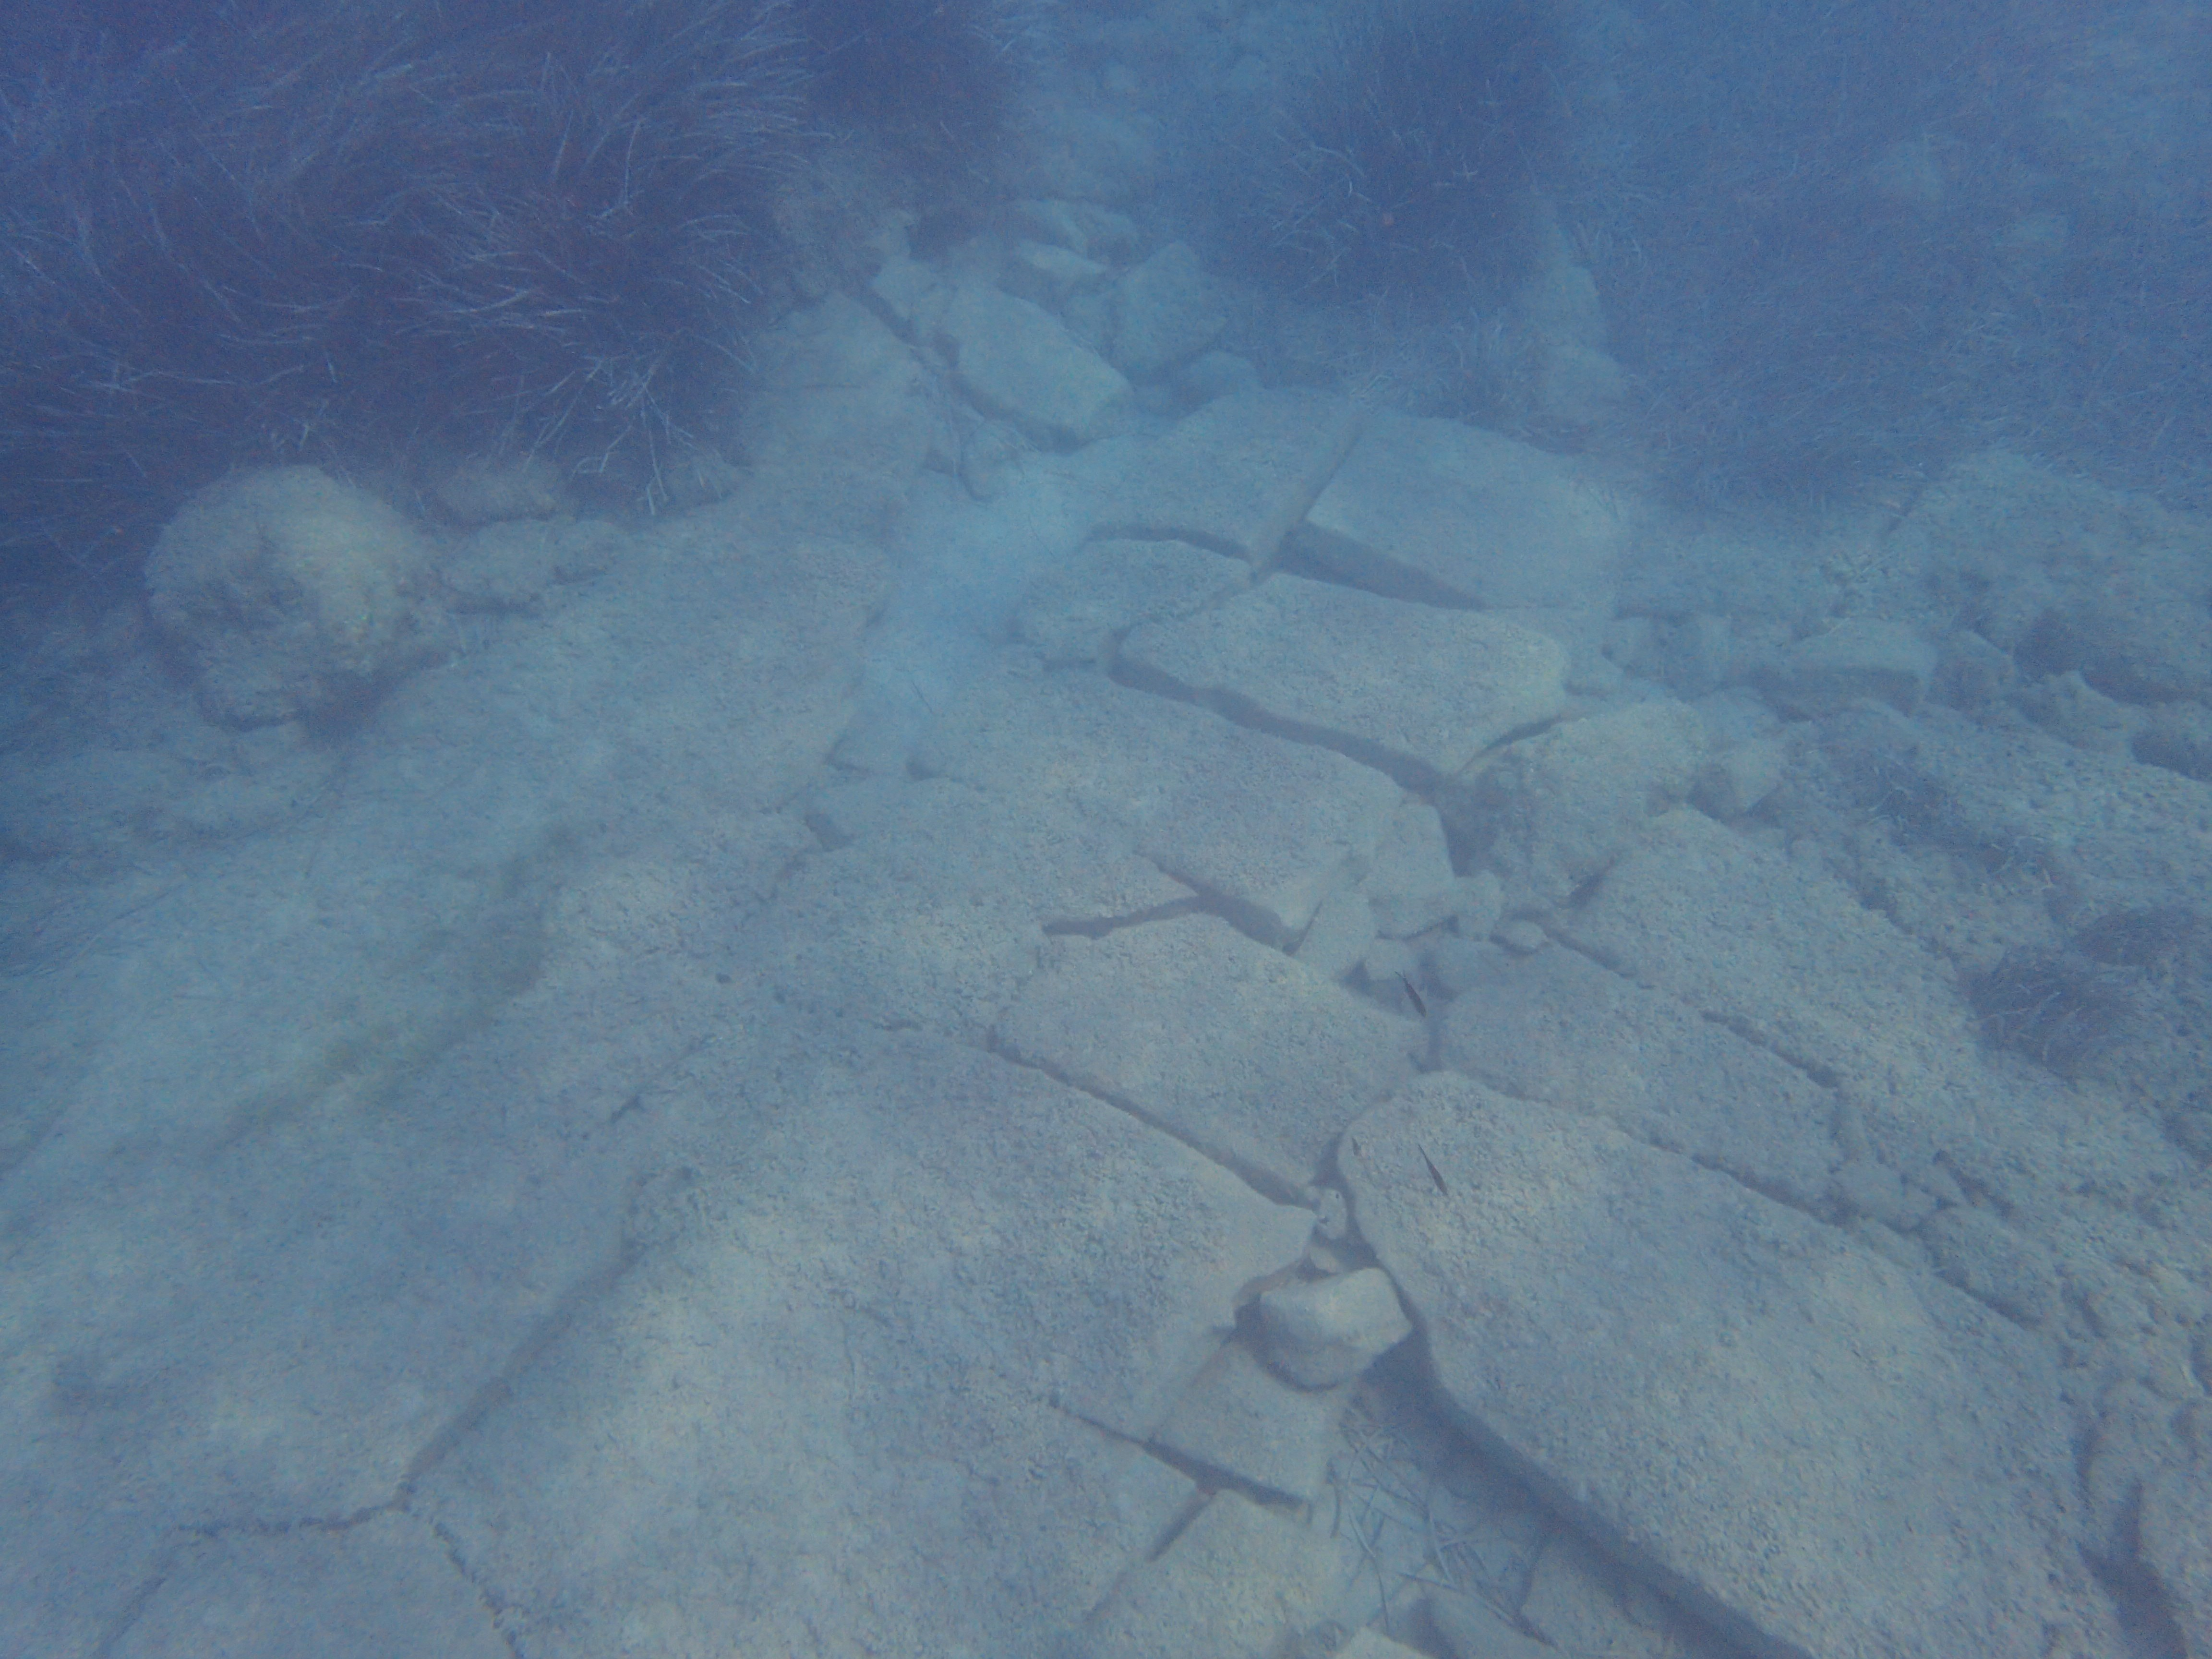
\includegraphics[width=\linewidth]{figures/takkou_dobroski_Fig2.jpg}
	\centering
	\caption{Possible underwater paved path or port related breakwater site, - \SI{8.5}{\metre} deep and \SI{20}{\metre} off shore. Photo taken by the author, directly facing north.}
	\label{fig:Takkou_Fig2}
\end{figure}

Following the cobbled section in Figure \ref{fig:Takkou_Fig2} directly north for about 15m led us to a wider and more complicated section, stretching out horizontally as far as the visibility allowed us to see (perhaps \SI{20}{\metre} either side). This section revealed circular ring shaped carved pieces of stone (See Fig. \ref{fig:Takkou_Fig3}). These rings protruded from the seabed and stand out in the natural marine environment as man-made. Perfectly spherical to the eye and a diameter of roughly \SI{1.5}{\metre}, we wondered whether these were Bronze Age stone anchors, but after coming across a better candidate for a stone anchor complete with rope wear (see Fig. \ref{fig:Takkou_Fig4}), we soon started to ask questions like “why would one waste time and resources carving a perfectly spherical anchor, and why are there so many in one location? Was this some type of anchorage site?”  

Pragmatically, there is no reason for a perfectly circular anchor – smooth and rounded surfaces allow for less friction on the seabed. However, it is possible that, under the marine growth attached to the stone, these rings are not perfectly circular and only appear to be so. With further research the exact dimensions can be fleshed out. So what are they? Since we counted nearly forty ‘rings’ around the entire site, we assessed the possibility that these had some function as mooring postholes but could not find other instances of Bronze Age mooring postholes in this region. Although at this stage of the research we cannot be entirely sure of what we have found, we are inclined to believe that what we have recorded are stone ring anchors.

%% this is figure 3
\begin{figure}
	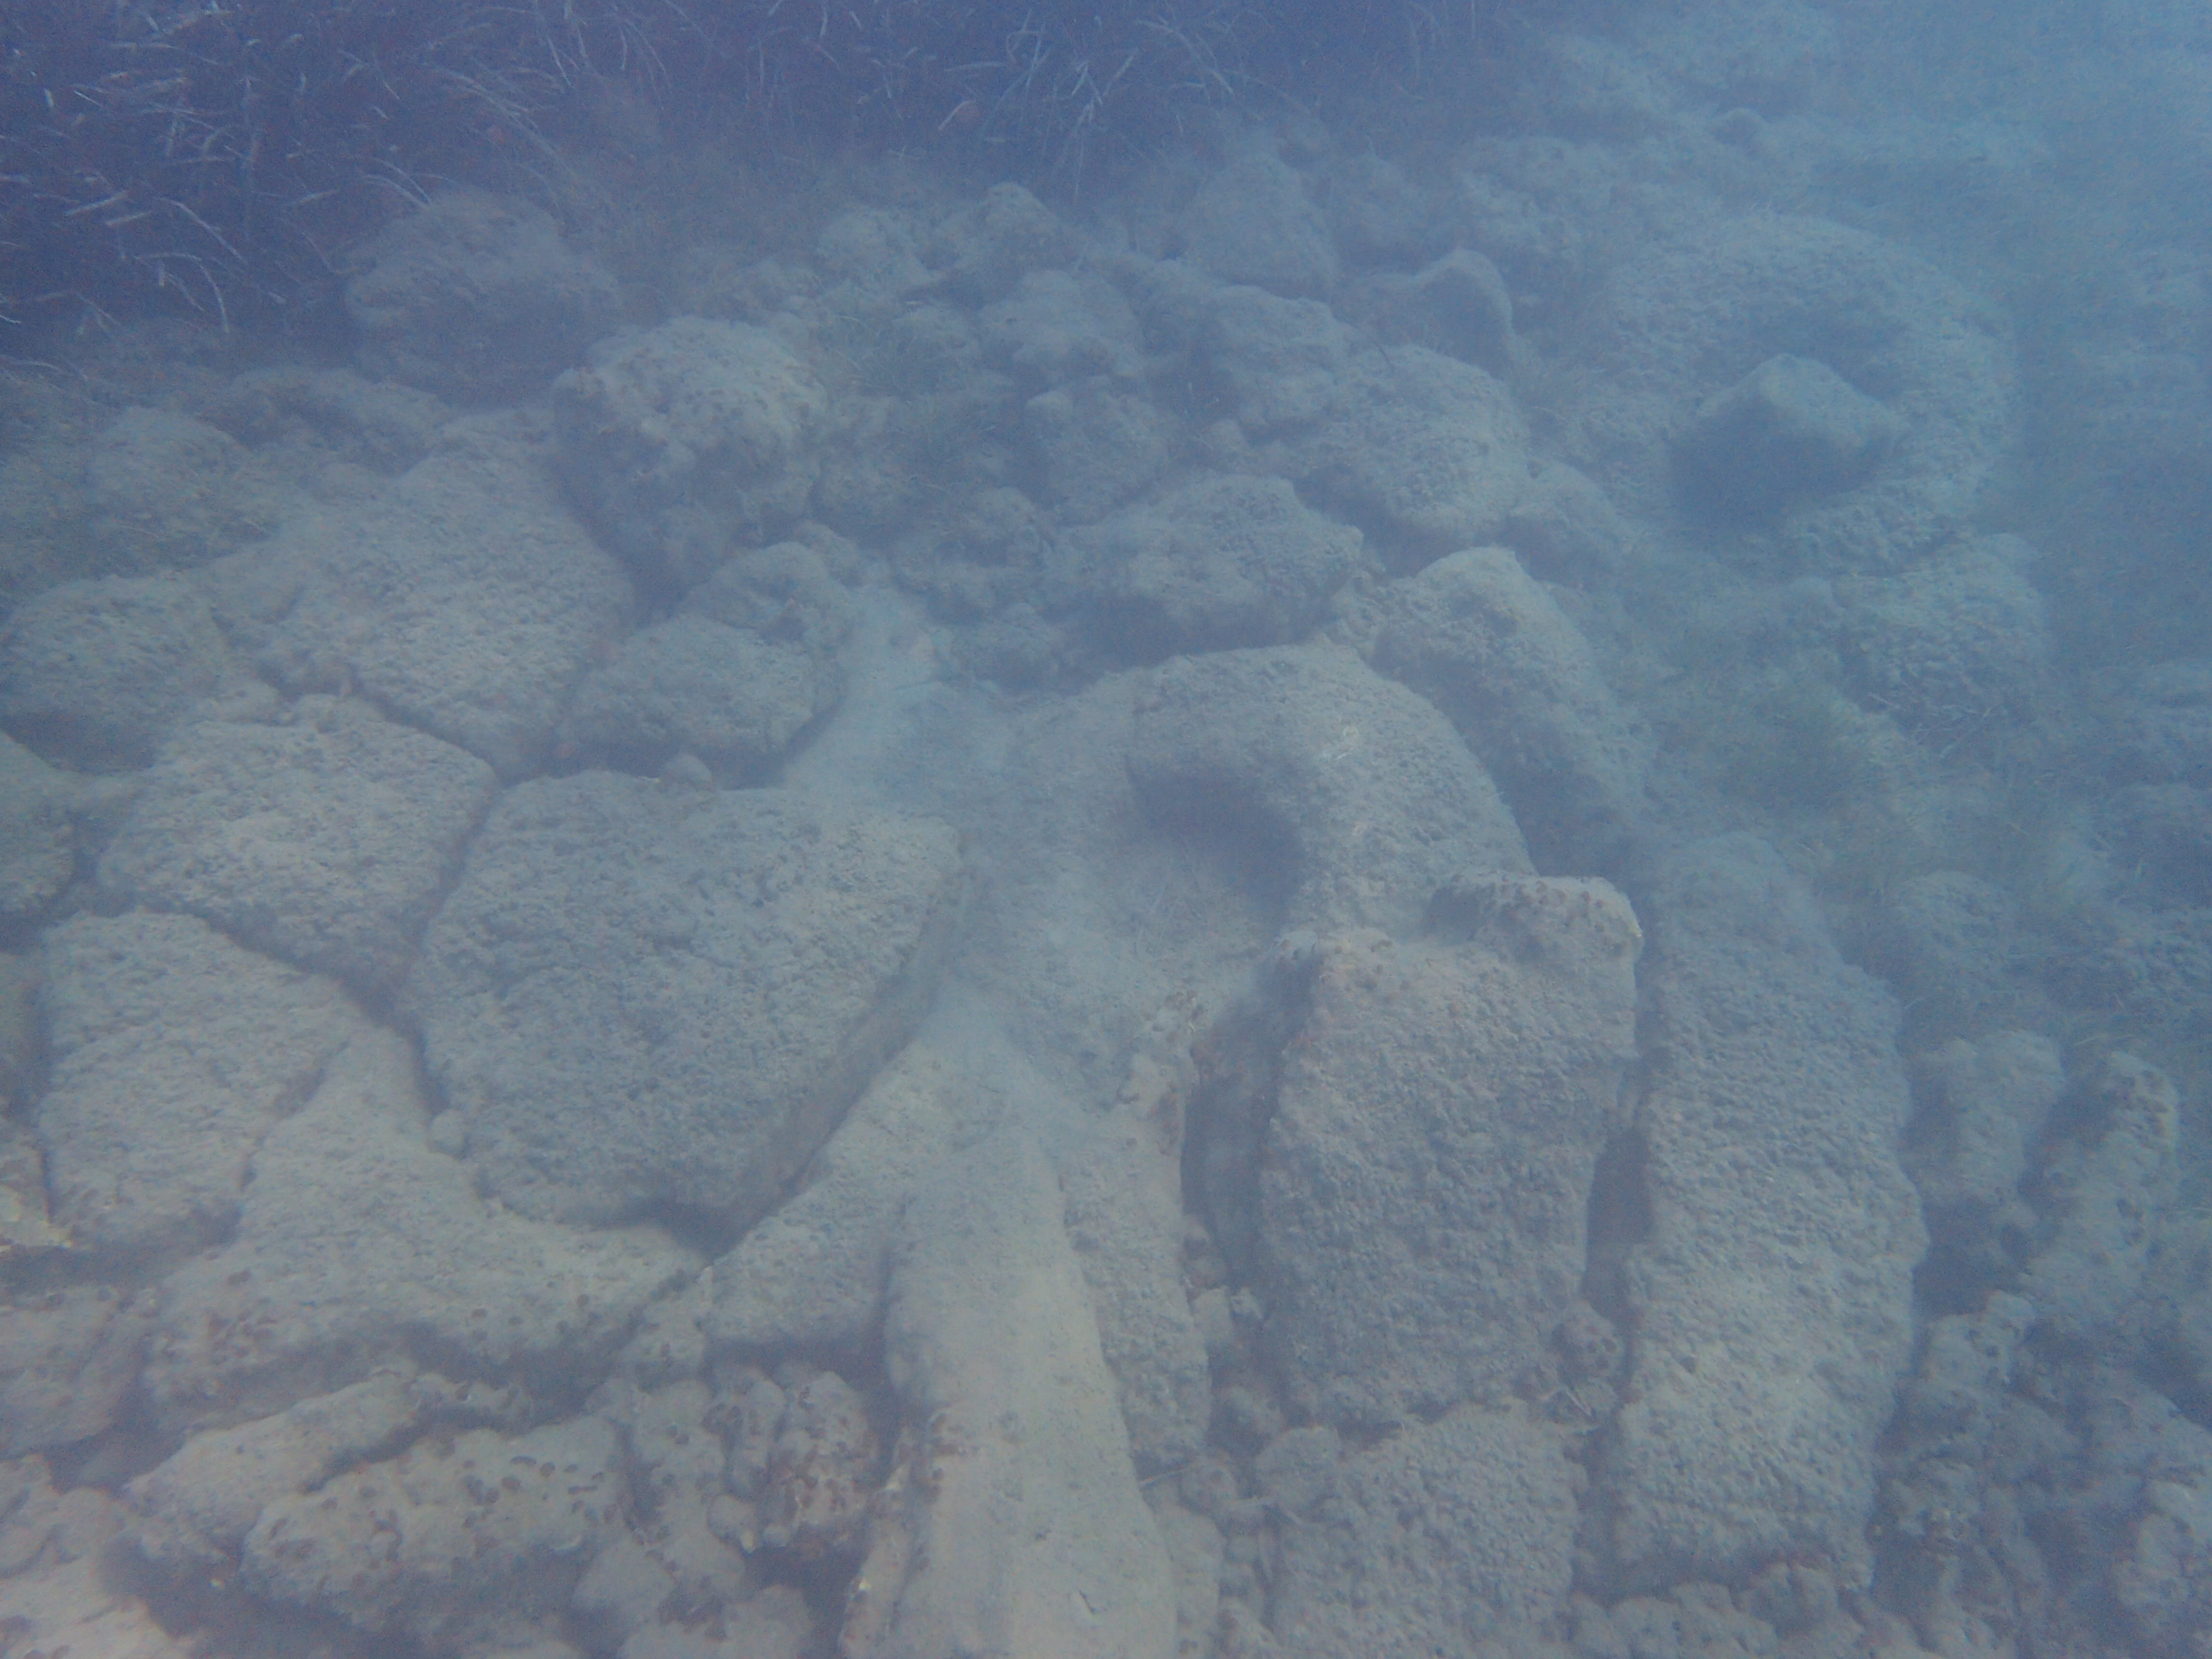
\includegraphics[width=\linewidth]{figures/takkou_dobroski_Fig3.jpg}
	\centering
	\caption{Two spherical stone ‘rings’, c.\SI{8.5}{\metre} deep – \SI{35}{\metre} offshore (photo taken by author).}
	\label{fig:Takkou_Fig3}
\end{figure}
	
%% this is figure 4
\begin{figure}
	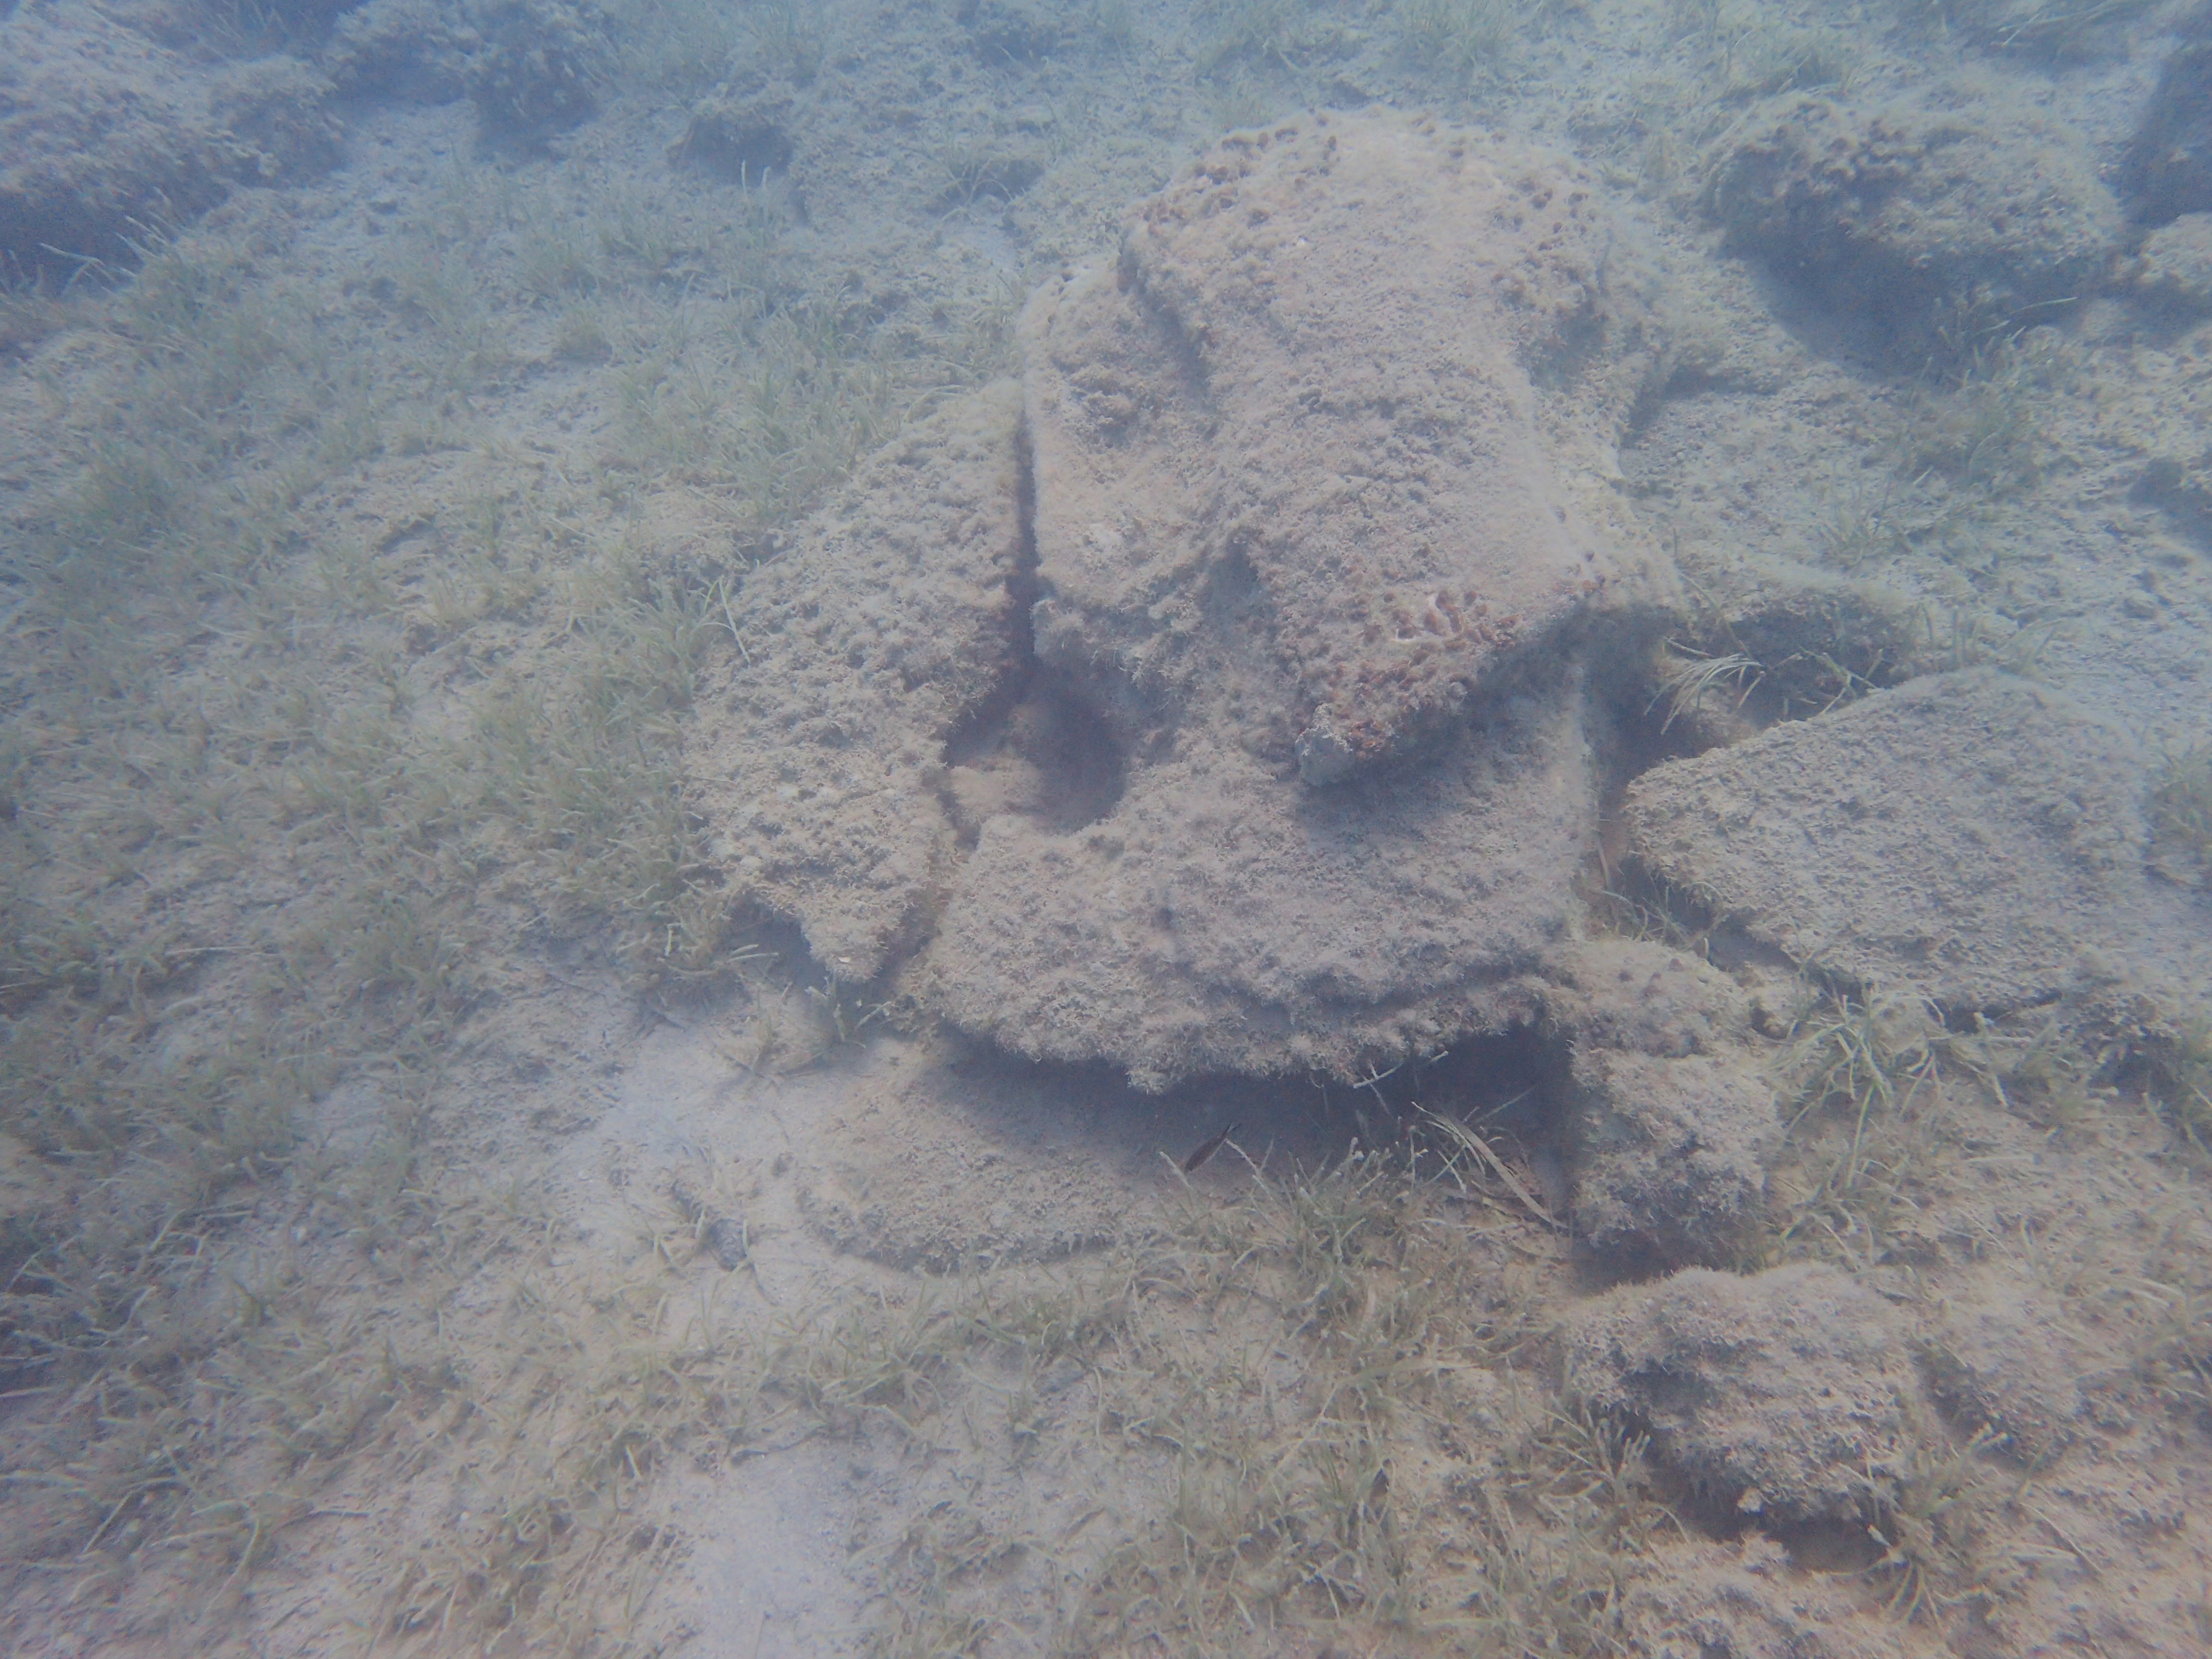
\includegraphics[width=\linewidth]{figures/takkou_dobroski_Fig4.jpg}
	\centering
	\caption{Stone anchor, c. \SI{9.5}{\metre} deep – \SI{40}{\metre} offshore (photo taken by author).}
	\label{fig:Takkou_Fig4}
\end{figure}		

After closer inspection of the ‘rings’ an issue with the anchorage/mooring station theory arose. There are in fact two typologies of ‘ring’ within this site, roughly split equally, 50/50, in terms of numbers of each type. The two types of ‘ring’ are found interspersed in the same locations and at similar depths. ‘Ring’ type II (see Figs. \ref{fig:Takkou_Fig5} \& \ref{fig:Takkou_Fig6}), is much more intricate in design and at first glance almost seems to be part of a much more grandiose site. 
	
%% this is figure 5
\begin{figure}
	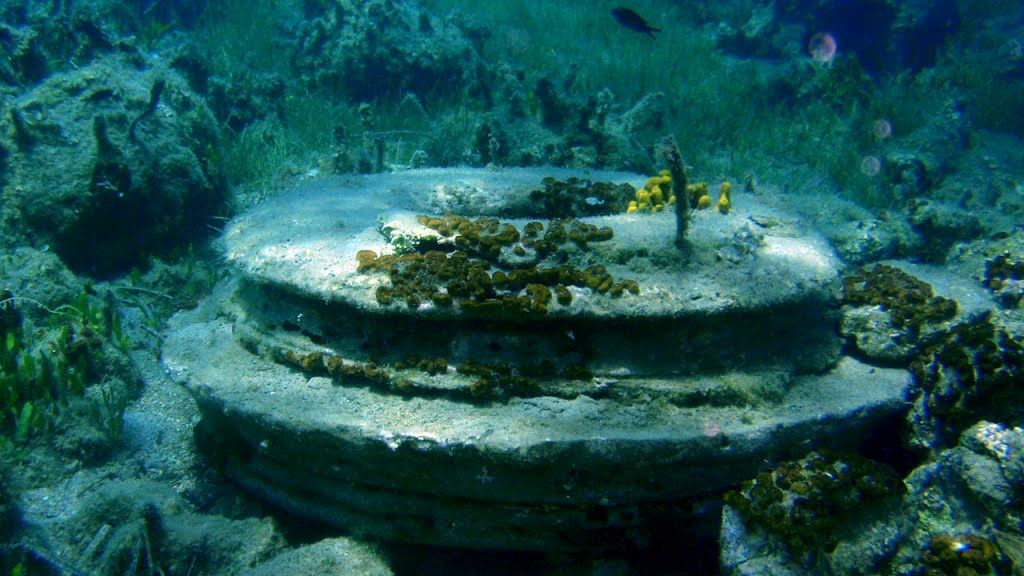
\includegraphics[width=\linewidth]{figures/takkou_dobroski_Fig5.jpg}
	\centering
	\caption{Spherical stone ‘ring’ type II, c. \SI{9}{\metre} deep -- \SI{35}{\metre} offshore (photo taken by author).}
	\label{fig:Takkou_Fig5}
\end{figure}

The sides of ‘ring’ type II have been delicately carved, which we can see from the photos but also by gently running ones fingers across the grooves in the stone. We have considered the possibility that ‘ring’ type II are the remnants of stone column bases. There is no doubt that aesthetics played a part in the making of this stone piece but, alas, at this preliminary stage we are currently not sure of its function. 

Indeed, this potential site is very interesting considering the fact that the last time it was above sea level was some 4000--6000 years ago \parencite{Flemming_2014} and the mystery surrounding the two types of spherical ‘rings’. Furthermore, the existence of a terrestrial site c.\SI{100}{\metre} away and \SI{120}{\metre} high on a hill aptly named ‘Pyrgo’, which can be translated as tower, overhanging and overlooking the possible port site, which begs the question: “are these two sites linked in some way?”
	
%% this is figure 6
\begin{figure}[!htb]
	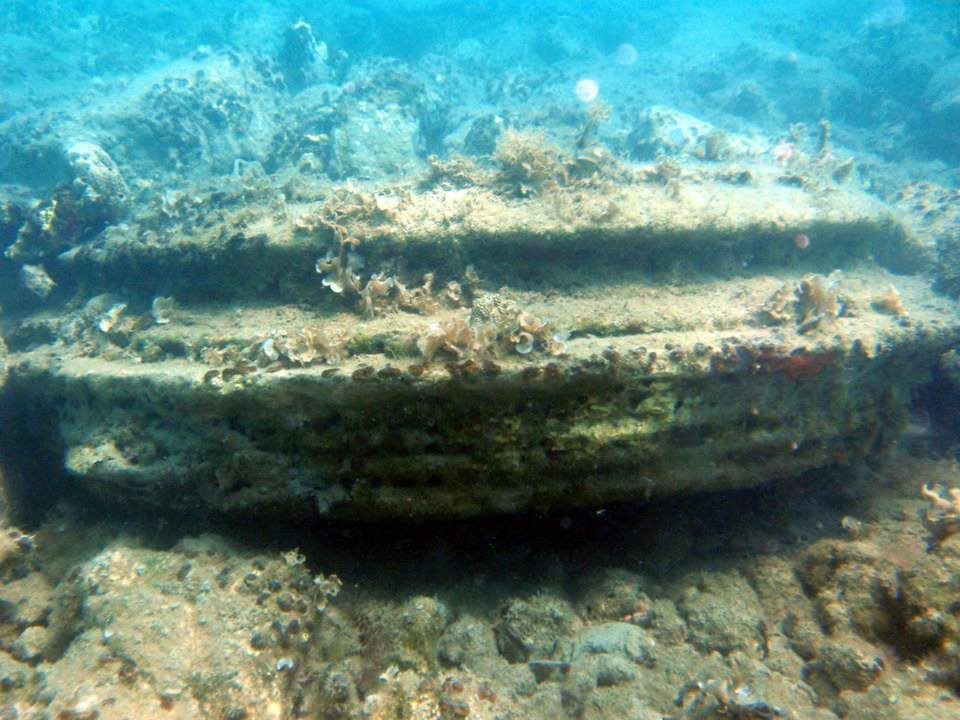
\includegraphics[width=\linewidth]{figures/takkou_dobroski_Fig6.jpg}
	\centering
	\caption{Spherical stone ‘ring’ type II side view, c.\SI{10}{\metre} deep – \SI{40}{\metre} offshore (photo taken by author).}
	\label{fig:Takkou_Fig6}
\end{figure}

Earlier in this section we mentioned a local historian we had encountered who was willing to help us garner ‘local knowledge’. The historian showed us his private collections from areas of the island he has visited and privately studied. Amongst his private collection were fragments of a Mycenaean terracotta stirrup jar, c.1200\BC. When asked where he had found the jar he told us of a hill perhaps only 100m away from the port site we had been visiting daily and directly overlooking it from a position of altitude. After some hours hiking we encountered a folklore favourite of the island – ‘Odysseus’ throne’, which is a rough stone seat made up of three different layers of stone and, amongst locals, historically associated with Odysseus. More important than the supposed ‘throne’ was the fact that it seemed to be flanked by a row of six rectangular \SI{2}{\metre} long stone slabs swallowed by the endless groves of olive trees (see Fig \ref{fig:Takkou_Fig7}; \ref{fig:Takkou_Fig9}).

We hypothesize that the terrestrial site is either the roofing slabs of a Mycenaean tomb or the foundation remnants of some type of building. The Mycenaean tomb implications further arose during the course of researching for this paper. \textcite{Agallopoulou_1973}'s tomb finds in the region of Keri were described as slabs of rock resting parallel with each other, and \textcite{Benton_1933} describes a different tomb find, “Near Mariais I saw a well preserved tomb, cut in soft psamitis (chalk) and roofed with five slabs, found in 1926. It is about 2 meters long..,” \parencite[21]{Benton_1933}. Figures \ref{fig:Takkou_Fig7} and \ref{fig:Takkou_Fig9} show six slabs laid out together on the top of a c.\SI{120}{\metre} hill overlooking what we believe to be a Bronze Age, or later, anchorage/port site. At this point any explanations attempting to link the two sites would be purely conjecture and more research needs to be conducted before any solid conclusions can be made. However, phenomenological approaches to these two sites beg a significant connection (especially if the date ranges turn out to be similar) as the port site is easily seen from the terrestrial hill site. It is almost as if the ‘throne’ looks over the harbor and the adjacent island.

%% this is figure 7
\begin{figure}[!p]
	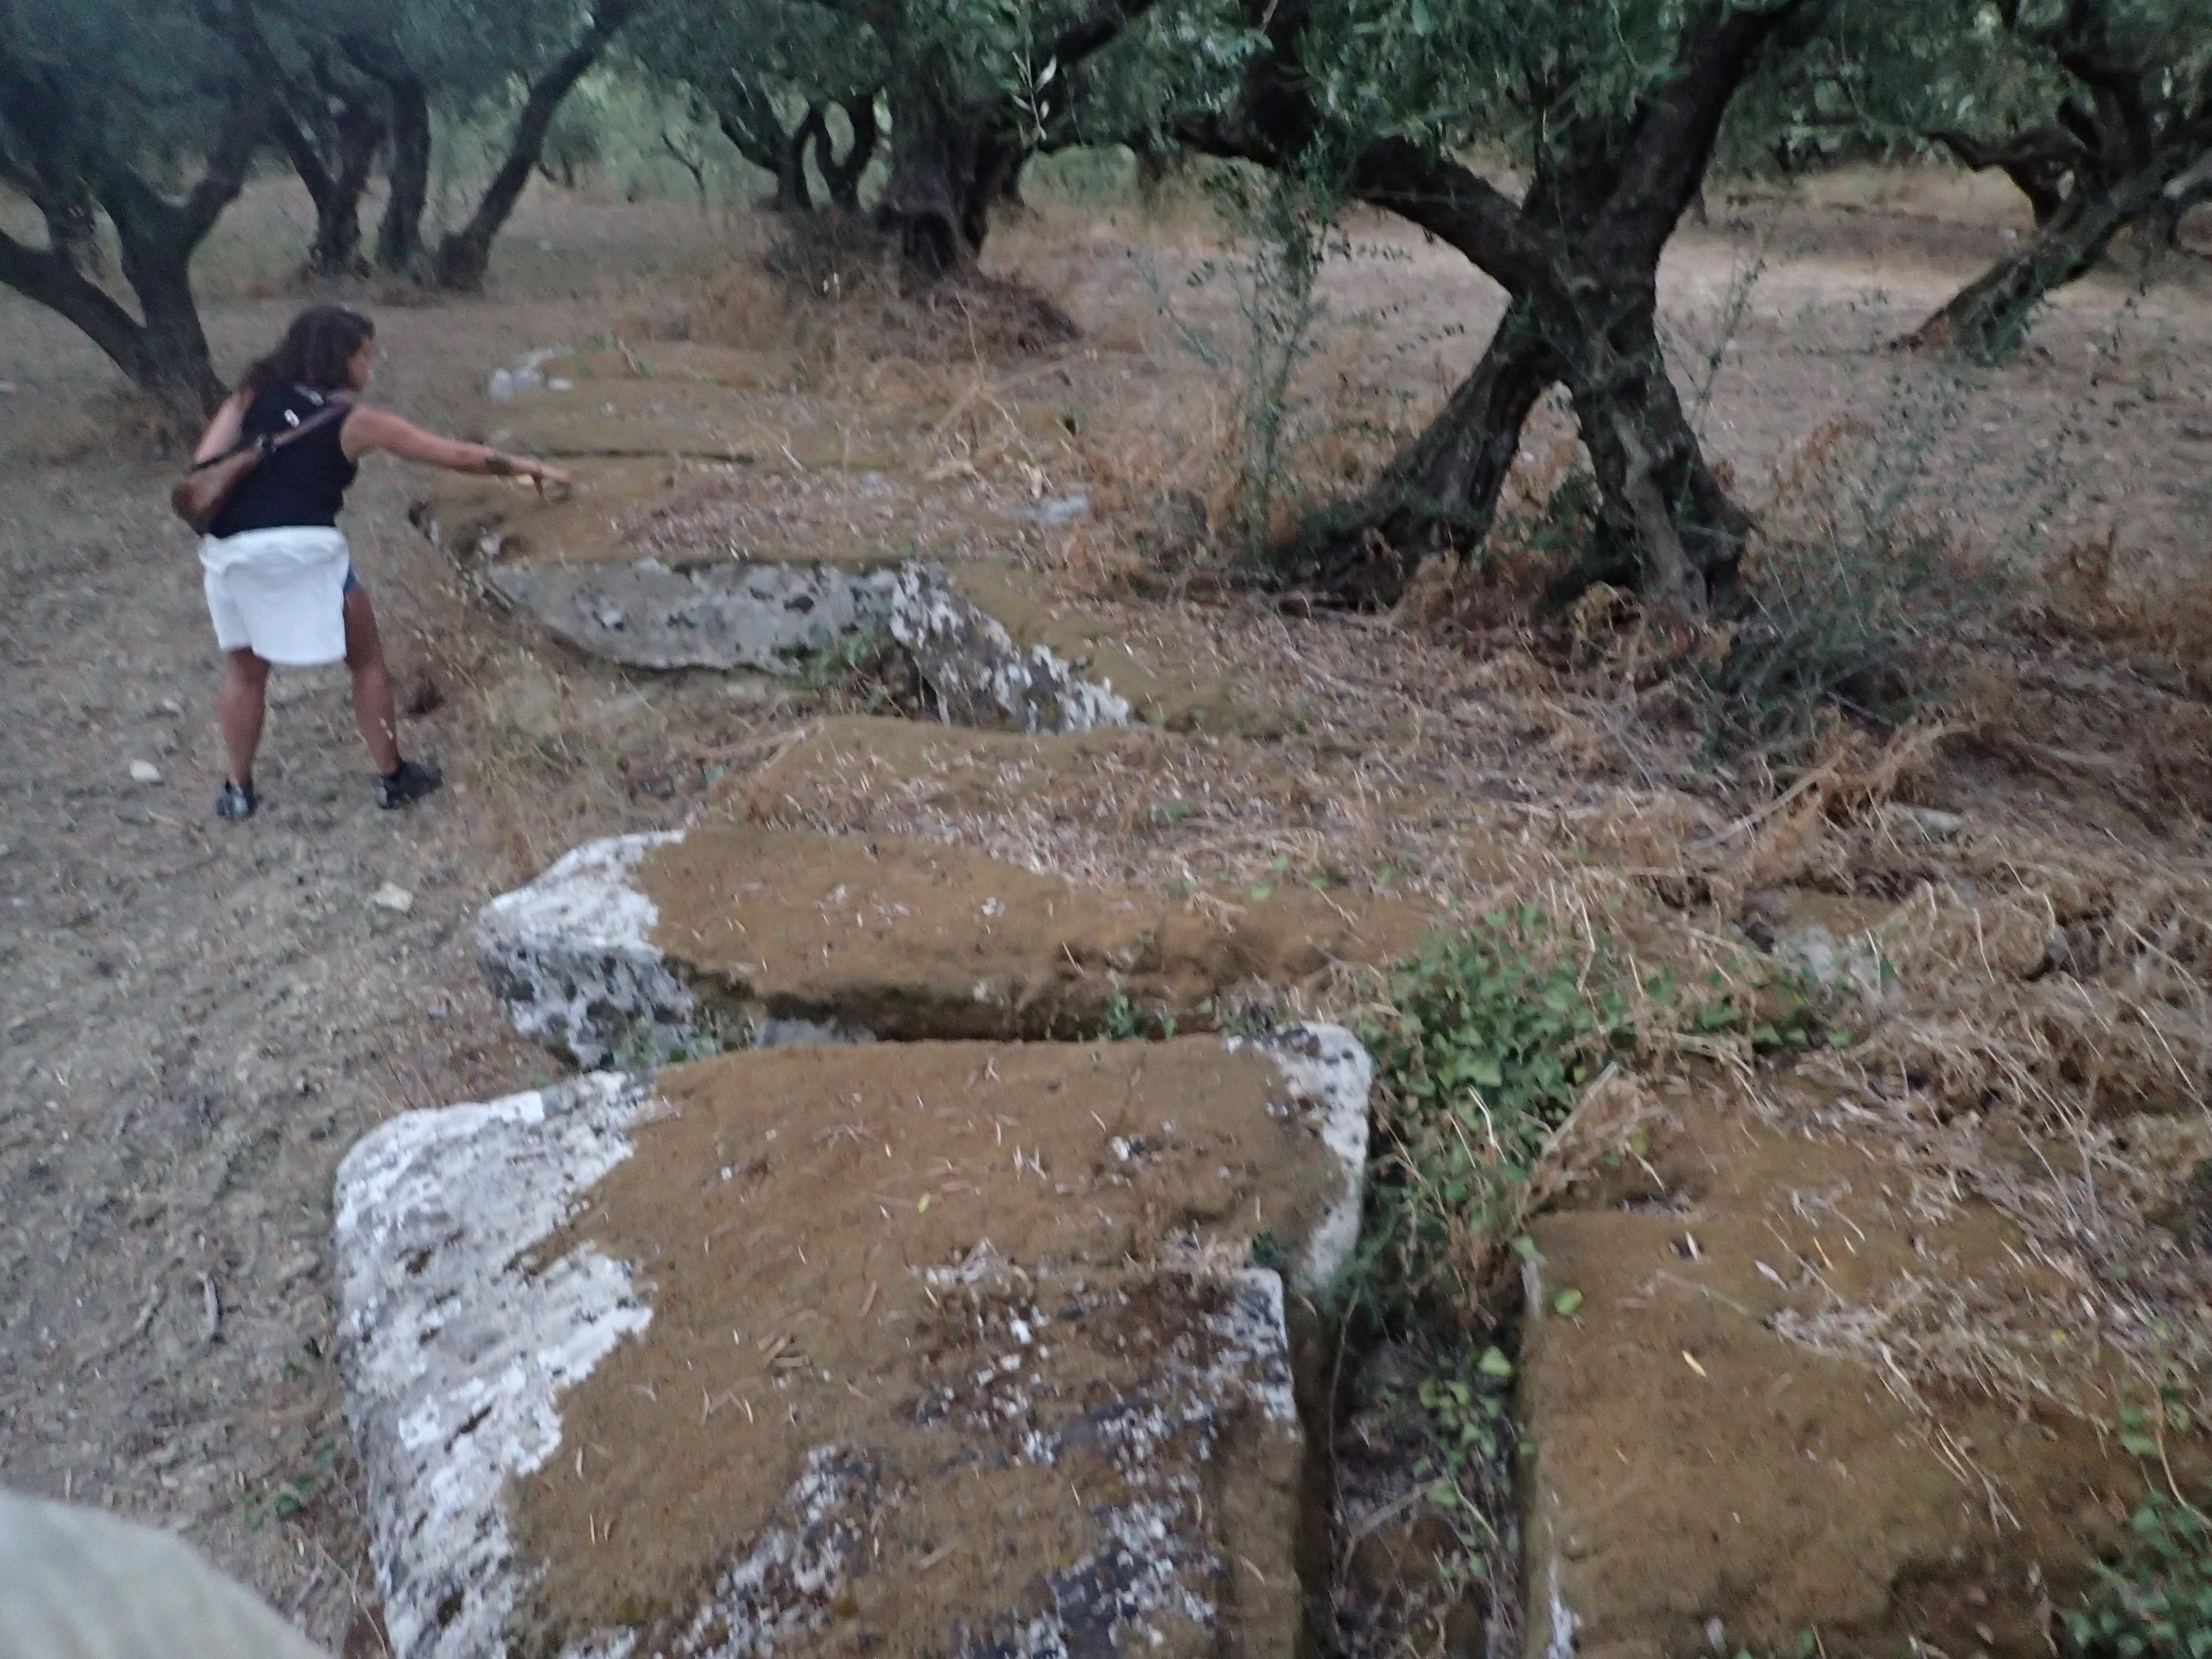
\includegraphics[width=.9\linewidth]{figures/takkou_dobroski_Fig7.jpg}
	\centering
	\caption{Six slabs laid together, viewed at a vertical angle and with first slab broken into two pieces and third slab missing just under half of its length (photo taken by author).}
	\label{fig:Takkou_Fig7}
\end{figure}

%% this is figure 8
\begin{figure}[!p]
	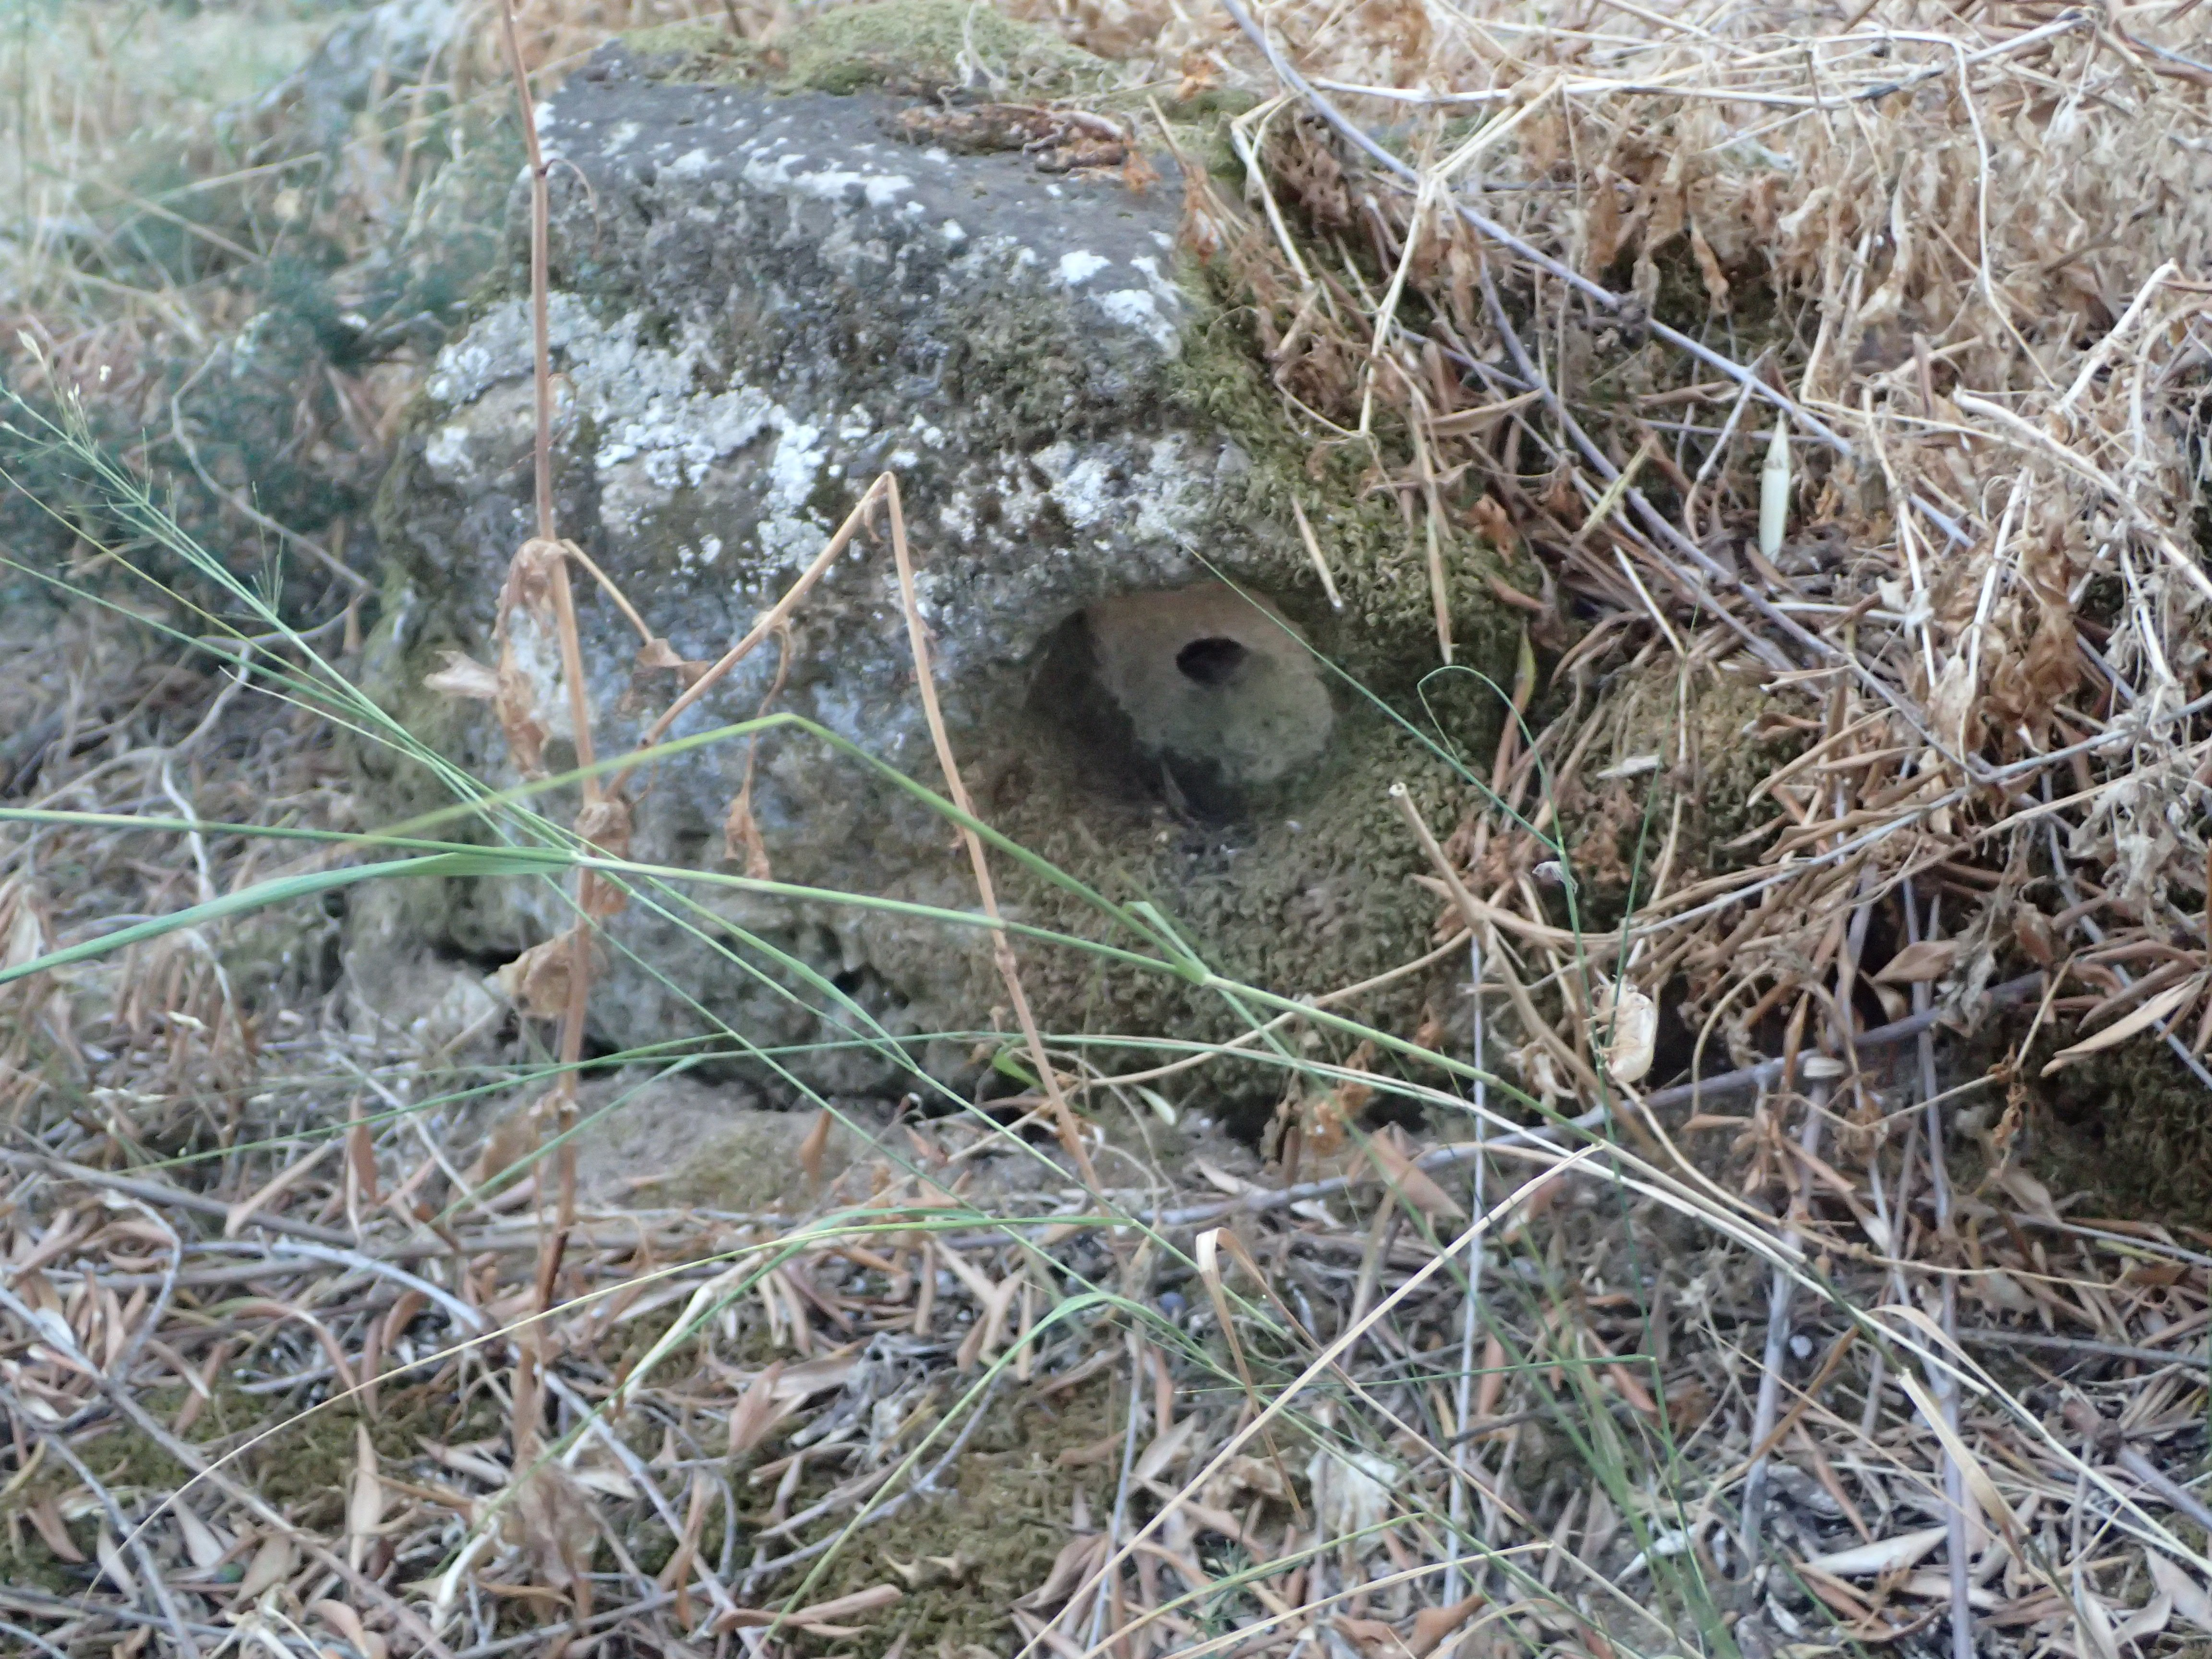
\includegraphics[width=.9\linewidth]{figures/takkou_dobroski_Fig8.jpg}
	\centering
	\caption{Perfectly circular hole found on the side of one of the six slabs (photo taken by author).}
	\label{fig:Takkou_Fig8}
\end{figure}

%% this is figure 9
\begin{figure}[!htb]
	\includegraphics[width=\linewidth]{figures/takkou_dobroski_Fig9.jpg}
	\centering
	\caption{Cross section of parallel slabs resting on a type of sandy/chalky bed (photo taken by author).}
	\label{fig:Takkou_Fig9}
\end{figure}

%\section{Conclusion}

\noindent The\marginnote{Conclusion} island’s archaeological record thus far suggests heavy Mycenaean use. \textcite{Benton_1933}'s discovery of Mycenaean houses and \textcite{Agallopoulou_1973}'s discovery of a Mycenaean cemetery further validates this connection. We know little about where Mycenaean anchorages and harbours were, or how they were used \parencite[1]{Tartaron_2013} and although much attention has been devoted to long-distance ‘international’ connections with the states, empires, and emporia of the eastern Mediterranean, comparatively little consideration has been extended to networks of maritime relations operating at a regional or micro scale. After recording and conserving, this type of question, indeed, lends itself to the scope of further research.

Planning for further research at the site is currently underway. We plan to return to both sites in order to survey the areas with more precision and completeness. For the underwater site the goal is to create a 3D photogrammetric mosaic of the seabed for a clearer and holistic view of the site, because for the moment, we are not sure how far out the port site extends itself into the sea. The terrestrial site is much more complicated in that the land is privately owned, and survey permits may be harder to obtain from the Hellenic Ministry of Culture because of this fact. We aim to have some agreement with the landowner in place and in time for a research start date of late next summer. 

The colourful and complicated history of Zakynthos presents interesting archaeological questions and problems. Community-inclusive methods have proven to be successful in overcoming some of these hurdles by providing new insights to the islands’ unique ancient landscape and the historical insight of local islanders.  From fishermen’s tales of net snagging to local inhabitants’ long-lived tales of Odyssean/ Mycenaean kingdoms, certainly, continuous in-depth exploration of the island is critical to produce a clearer understanding of ancient occupation in the region. Due to substantial archaeological fragmentation, this investigation includes gaining a deeper sense of the local communities interaction with the ancient heritage of the island; researching knowledge of known sites (both intact and destroyed), locating artifacts held in private collections, and recording local folklore. The two potential sites presented in this paper merit further research, and may prove to be connected. The difficult archaeological terrain of Zakynthos requires archaeologists to produce a full arsenal of tools, theories, and methods to illuminate the island’s past.

\myseparator
\begin{myabstract}
\foreignlanguage{greek}{Η αρχαιολογία της Ζακύνθου είναι αραιά σε σχέση με εκείνη των άλλων Ιόνιων Νήσων. Αυτό οφείλεται σε μια ποικιλία περιστάσεων - την έλλειψη αρχαιολογικής έρευνας και τον ψηλό βαθμό καταστροφής που οφείλεται σε ένα συνδυασμό πολέμου, σεισμική δραστηριότητας, καθώς και εντατική χρήση της γής για ανάπτυξη, η οποία έχει ως αποτέλεσμα την απώλεια ενός άγνωστου αριθμού αρχαιολογικών τόπων και έργα τέχνης. Ως αποτέλεσμα αυτής της απώλειας, τα αρχαιολογικά έργα στο νησί της Ζακύνθου έχουν δημιουργήσει μια σειρά από ασκήσεις επί χάρτου, οι οποίες έχουν αποδειχθεί ανεπαρκής για την εξακρίβωση μια ολοκληρωμένης προϊστορικής ερμηνείας του νησιού. Η παρούσα έρευνα εστειάζει στην αρχαιολογική ιστορία του νησιού και παρουσιάζει αποτελέσματα έρευνας. Η έρευνα έχει την υποστήριξη της έρευνας DPhil για το έτος 2016, και πραγματοποιήθηκε τον Αύγουστο του 2015 από συγγραφείς στην παραθαλάσια περιοχή του Κατασταρίου της Ζακύνθου (Ελλάδα). Επιπλέον, αυτό το έγγραφο αποτελεί μια απάντηση για την δύσκολη αρχαιολογική ζώνη του νησιού με τη διερεύνηση των δυνατοτήτων μιας νέας κοινότητας χωρίς αποκλεισμούς στην μεθοδολογία έρευνας για την περιοχή.}

\keywords[λέξεις-κλειδιά]{Ζάκυνθος, Καταστάρι, Έρευνα, Προφορική Ιστορία, Προϊστορία, Τοπίο αρχαιολογία.}
\end{myabstract}
\printbibliography[heading=subbibnumbered] 
\label{Takkou:lastpage}
\closingarticle
